\section{Thực nghiệm đa agent trong thị trường mô phỏng}
\subsection{Mục tiêu và nguồn thực nghiệm}
Thực nghiệm AGENT 02 khảo sát hai người bán cạnh tranh: một agent dùng Q-learning và một agent thực hiện luật cố định. Mục tiêu là so sánh lợi nhuận, hành vi giảm giá và khả năng thích nghi khi mức chiết khấu thay đổi. Kết quả trong phần này được tổng hợp từ báo cáo thực hành AGENT 02 của Kiều Trường Giang, B23DCCN254, cùng các tệp kết quả đã lưu. Dữ liệu là quỹ đạo sinh bởi mô phỏng, không phải giao dịch thương mại thực.

\subsection{Quan sát, hành động và phần thưởng}
Trạng thái cục bộ của người bán $i$ là $s_i(t)=(d_t,c_i(t))$, trong đó nhu cầu $d_t\in\{0,1\}$ và $c_i(t)$ là hành động ở bước trước của đối thủ. Hành động $a_i(t)=0$ biểu thị giữ giá, $a_i(t)=1$ biểu thị giảm giá. Hai agent quyết định trước khi môi trường tính kết quả, nên không agent nào được quan sát trước lựa chọn hiện tại của đối thủ.

Xác suất chuyển đổi và lượng bán được mô tả bởi
\[
p_i(t)=\operatorname{clip}\left(0.30+0.25d_t+0.15a_i(t)-0.10a_{-i}(t),0.05,0.95\right),
\]
\[
S_i(t)\sim\operatorname{Binomial}(N_t,p_i(t)),\qquad
r_i(t)=S_i(t)\left[P(1-\delta a_i(t))-C\right].
\]
Số khách tiềm năng $N_t$ bằng 10 hoặc 20 tùy nhu cầu; giá gốc $P=10$, chi phí $C=5$, chiết khấu mặc định $\delta=0,20$. Phần thưởng là lợi nhuận nên tăng doanh số không nhất thiết làm tăng reward. Lượng bán của hai người được lấy mẫu riêng, không bị buộc có tổng thị phần bằng một; đây là một giả định đơn giản hóa của môi trường.

\subsection{Hai cơ chế quyết định}
Agent RL dùng bảng Q gồm bốn trạng thái và hai hành động. Agent theo luật giảm giá khi và chỉ khi nhu cầu cao, đồng thời đối thủ đã giảm giá ở bước trước:
\[
\pi_{\mathrm{rule}}(d,c)=\begin{cases}1,&d=1\ \text{và}\ c=1,\\0,&\text{các trường hợp khác}.\end{cases}
\]
Khi khởi tạo episode, hành động trước của cả hai bằng không. Cấu hình này có thể duy trì quỹ đạo cùng giữ giá nếu agent RL không tạo kích thích thay đổi. Reward của mỗi agent phụ thuộc hành động của bên còn lại, vì vậy đây là môi trường đa agent dù chỉ có một agent cập nhật chính sách trong thí nghiệm chính.

\section{Quy trình huấn luyện và đánh giá}
\subsection{Cấu hình và phân tách train--eval}
\begin{table}[H]\centering\small\caption{Cấu hình thực nghiệm AGENT 02.}\begin{tabular}{p{7cm}p{6cm}}\toprule Thành phần & Giá trị\\\midrule
Episode huấn luyện / số bước mỗi episode & 5.000 / 20\\
Episode đánh giá / tổng bước & 500 / 10.000\\
Tốc độ học $\alpha$ / hệ số chiết khấu $\gamma$ & 0,10 / 0,90\\
Khám phá ban đầu / tối thiểu / suy giảm & 0,20 / 0,02 / 0,995\\
Seed baseline train / eval & 42 / 500042\\
Năm seed huấn luyện lặp lại & 11, 22, 33, 44, 55\\
Seed đánh giá lặp lại & Seed train cộng 800000\\\bottomrule\end{tabular}\end{table}
Mỗi cấu hình có 100.000 bước huấn luyện. Trong đánh giá, bảng Q giữ cố định, tắt nhánh khám phá và không gọi hàm học. Bộ sinh số ngẫu nhiên của môi trường và của bộ chọn hành động được tách riêng. Cùng seed giúp tái lập nhưng không bảo đảm hai chính sách khác nhau tiêu thụ đúng cùng chuỗi số ngẫu nhiên khi tham số lấy mẫu thay đổi.

\subsection{Chỉ số và các yếu tố khảo sát}
Lợi nhuận trung bình mỗi bước là $\bar R_i=T^{-1}\sum_{t=1}^{T}r_i(t)$. Tỷ lệ giảm giá $\rho_i$ bằng số lần chọn hành động một chia cho $T$. Chỉ số thứ nhất đánh giá kết quả; chỉ số thứ hai giúp giải thích hành vi tạo ra kết quả đó. Với nhiều seed, báo cáo trung bình và độ lệch chuẩn mẫu của $\bar R_i$.

Các nhóm thí nghiệm lần lượt thay đổi tốc độ học, lịch khám phá và mức chiết khấu. Với tốc độ học, so sánh $\alpha=0,01;0,10;0,50$ trong cùng nhóm seed. Với khám phá, khảo sát các lịch giảm dần và mức cố định. Với chuyển môi trường, so sánh chính sách học ở chiết khấu 20\% khi đưa sang 5\%, có và không huấn luyện lại.
\section{Kết quả và nhận xét}
\subsection{Cấu hình cơ sở và nhiều seed}
Ở baseline, RL đạt reward trung bình 35,1275 mỗi bước, agent theo luật đạt 34,9685. Cả hai cùng giữ giá trong toàn bộ 10.000 bước đánh giá. Do hành vi giống nhau, chênh lệch nhỏ trong reward phản ánh phần ngẫu nhiên của lượng bán, không đủ để kết luận RL có chính sách tốt hơn.
\begin{table}[H]\centering\small\caption{Reward mỗi bước qua năm seed của cấu hình chiết khấu 20\%.}\begin{tabular}{rrrr}\toprule Seed & Q-learning & Theo luật & Chênh lệch\\\midrule
11 & 34.7440 & 34.8265 & -0.0825\\
22 & 35.3250 & 35.2945 & 0.0305\\
33 & 34.6725 & 34.7115 & -0.0390\\
44 & 35.1165 & 35.0835 & 0.0330\\
55 & 34.6015 & 34.7445 & -0.1430\\\midrule
Trung bình & 34.8919 & 34.9321 & -0.0402\\
SD mẫu & 0.3132 & 0.2496 & 0.0754\\\bottomrule\end{tabular}\end{table}
Kết quả trung bình của RL thấp hơn 0,0402 điểm mỗi bước. Ba seed cho chênh lệch âm, hai seed cho chênh lệch dương. Bảng không cho thấy ưu thế nhất quán của RL trong cấu hình gốc; luật đơn giản đã đạt hành vi phù hợp với môi trường đang xét.
\begin{figure}[H]\centering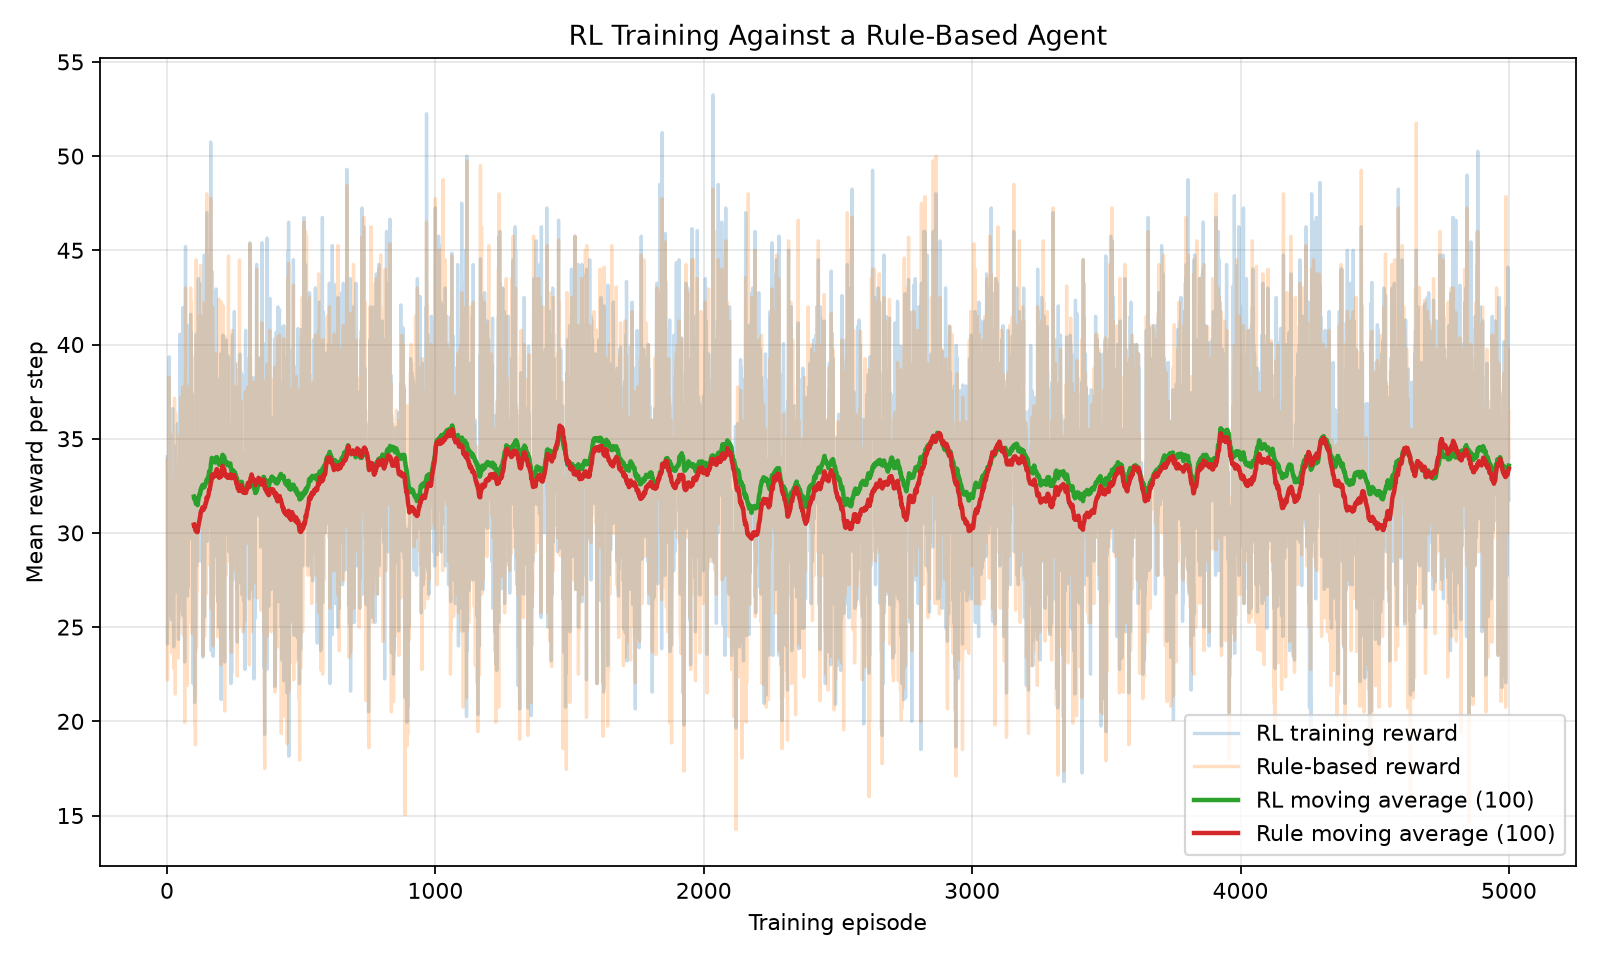
\includegraphics[width=\linewidth,height=.43\textheight,keepaspectratio]{figures/agent02-episode_rewards.png}\caption{Reward theo episode trong kết quả thực hành AGENT 02 đã lưu.}\end{figure}
\subsection{Ảnh hưởng của tốc độ học và khám phá}
Với seed train 1042 và eval 600042, hai mức $\alpha=0,01$ và $0,10$ cùng cho reward RL là 35,2475; mức $0,50$ cho 28,5085 và chọn giảm giá ở 40,52\% bước đánh giá. Tốc độ cập nhật lớn hơn không tự bảo đảm chính sách tốt hơn: bảng Q có thể biến động mạnh trước reward ngẫu nhiên, làm agent chuyển sang hành vi có lợi nhuận thấp hơn.
\begin{figure}[H]\centering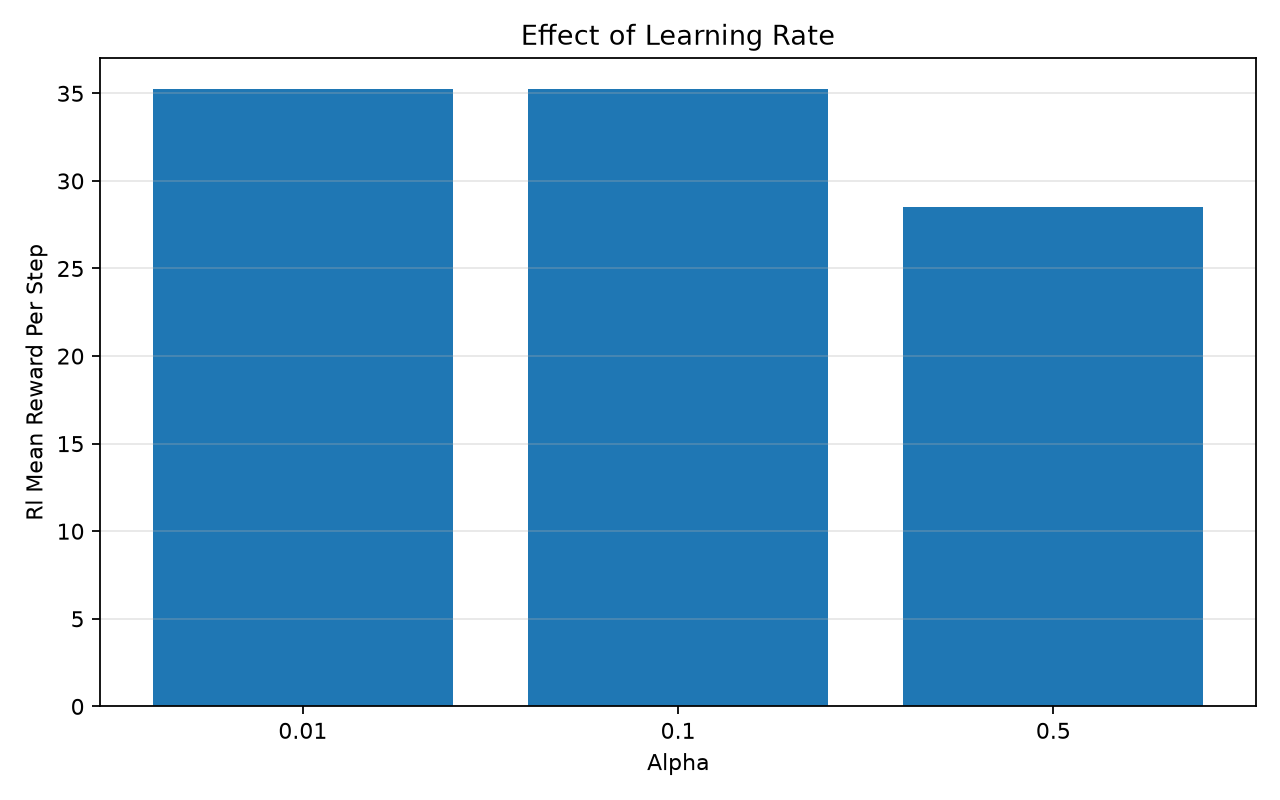
\includegraphics[width=.95\linewidth,height=.38\textheight,keepaspectratio]{figures/agent02-learning_rate_comparison.png}\caption{Đối chiếu các tốc độ học trong cùng nhóm thực nghiệm.}\end{figure}
Khám phá cần được phân biệt giữa pha học và pha sử dụng chính sách. Reward thu được khi còn chọn hành động ngẫu nhiên không phải chất lượng của chính sách sau huấn luyện. Các lịch khám phá vì vậy phải được đánh giá lại khi tắt khám phá, thay vì chỉ so sánh tổng reward trong train.
\begin{figure}[H]\centering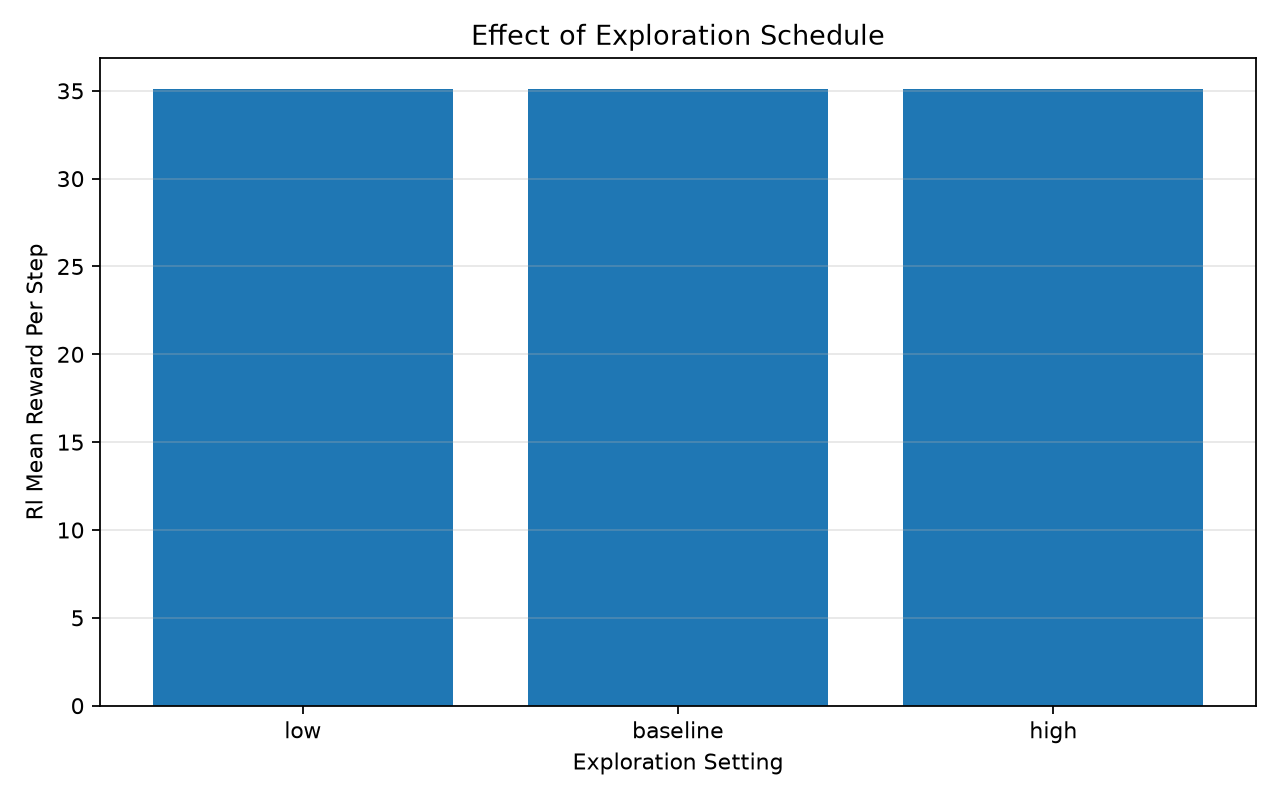
\includegraphics[width=.95\linewidth,height=.38\textheight,keepaspectratio]{figures/agent02-exploration_comparison.png}\caption{Kết quả các cấu hình khám phá trong báo cáo AGENT 02.}\end{figure}
\subsection{Chuyển môi trường và huấn luyện lại}
\begin{table}[H]\centering\small\caption{Thay đổi chiết khấu: trung bình reward và SD mẫu qua năm seed.}\begin{tabular}{llrrr}\toprule Điều kiện & Agent & Trung bình & SD & Giảm giá\\\midrule
20\%, gốc & RL & 34.8919 & 0.3132 & 0.00\%\\
20\%, gốc & Theo luật & 34.9321 & 0.2496 & 0.00\%\\
5\%, đóng băng & RL & 34.8919 & 0.3132 & 0.00\%\\
5\%, đóng băng & Theo luật & 34.9321 & 0.2496 & 0.00\%\\
5\%, học lại & RL & 36.7892 & 0.5834 & 76.54\%\\
5\%, học lại & Theo luật & 32.1593 & 0.3058 & 36.27\%\\\bottomrule\end{tabular}\end{table}
Khi chính sách cũ giữ nguyên và không giảm giá, thay đổi $\delta$ không ảnh hưởng giá thực nhận trên các bước quan sát nên reward giữ nguyên. Sau khi được học lại ở mức 5\%, RL giảm giá thường xuyên hơn và đạt trung bình 36,7892. Kết quả này phản ánh khả năng tìm chính sách mới khi được huấn luyện trong môi trường đã đổi, không phải khả năng tự thích nghi của một bảng Q đóng băng.
\begin{figure}[H]\centering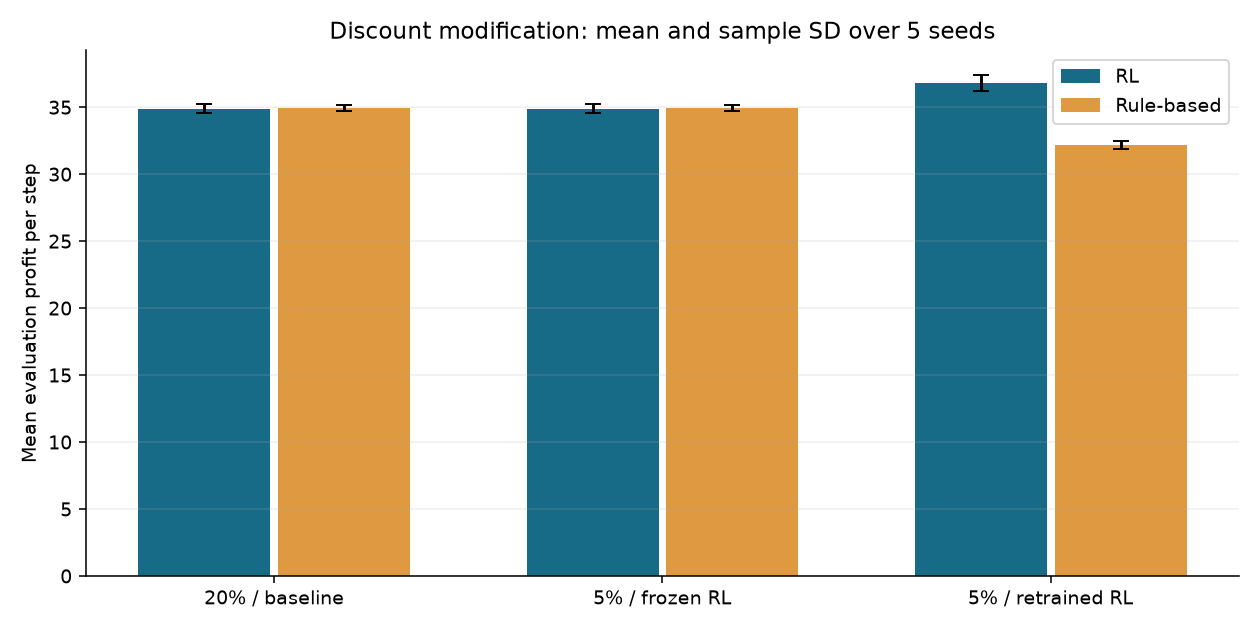
\includegraphics[width=\linewidth,height=.42\textheight,keepaspectratio]{figures/agent02-robustness.png}\caption{Đối chiếu chính sách gốc, chính sách đóng băng và chính sách học lại khi giảm chiết khấu.}\end{figure}
\section{Tái lập, giới hạn và tiểu kết}
\productlink{Mã và dữ liệu thực nghiệm AGENT 02}{https://github.com/jellalaz/He_Thong_Thong_Minh_Thay_Que/tree/main/experiments/agent02}
Tệp \path{experiments/agent02/data/all_evaluations.csv} lưu kết quả từng cấu hình, seed và agent. Mã trong thư mục \path{experiments/agent02/code/} mô tả môi trường và quy trình thực nghiệm. Các bảng trung bình được đối chiếu lại từ CSV; chúng là kết quả của bài thực hành đã lưu, không phải số liệu lấy từ báo cáo của sinh viên khác.

Mô phỏng có không gian trạng thái nhỏ, đối thủ theo luật cố định và nhu cầu được sinh đơn giản. Các giả định này làm bài toán thuận tiện để phân tích nhưng hạn chế khả năng khái quát sang thị trường thật. Khi cả hai agent cùng học, mỗi agent phải đối mặt với môi trường thay đổi do chính sách đối thủ; thí nghiệm chính chưa kiểm chứng điều kiện đó.

So sánh cho thấy lựa chọn giữa luật và học phải dựa trên mục tiêu, cấu trúc môi trường và bằng chứng đánh giá. Luật cố định có thể đủ tốt ở một cấu hình; học tăng cường có ích khi cấu trúc phần thưởng thay đổi và có dữ liệu tương tác để học lại. Đánh giá cần báo cáo cả lợi nhuận, hành vi và giả thiết quan sát, thay vì chỉ nêu agent nào có reward lớn hơn.
